\documentclass[conference]{IEEEtran}
\usepackage{cite}
\usepackage{amsmath}
\usepackage{algorithmic}
\usepackage{array}
\usepackage{url}
\usepackage{graphicx}
% correct bad hyphenation here:
\hyphenation{op-tical net-works semi-conduc-tor}


\begin{document}
% paper title
\title{Wireless networks based on context-aware routing:\\an Internet of Things application}

% author names and affiliations
\author{\IEEEauthorblockN{Victor\IEEEauthorrefmark{1},
Luiz Oliveira\IEEEauthorrefmark{1},
Jorge Guilherme\IEEEauthorrefmark{1},
Kim M. Mota\IEEEauthorrefmark{1},
Wanessa de A. Silva\IEEEauthorrefmark{2},
\\
Raquel Gonçalves\IEEEauthorrefmark{2},
Larinni M.\IEEEauthorrefmark{2},
Joao\IEEEauthorrefmark{2},
Diego\IEEEauthorrefmark{3},
Maira\IEEEauthorrefmark{3} and
Sergio\IEEEauthorrefmark{3}}
\IEEEauthorblockA{\IEEEauthorrefmark{1}Department of Electrical Engineering\\
University of Brasilia,
Brasilia, Brazil 30332--0250\\ Email: xxx@unb.br}
\IEEEauthorblockA{\IEEEauthorrefmark{2}Department of XXXX\\
University of Brasilia,
Brasilia, Brazil \\ Email: xxx@iee}
\IEEEauthorblockA{\IEEEauthorrefmark{3}Department of Electrical Engineering\\
University of Brasilia,
Brasilia, Brazil \\ Email: yyy@iee}}

% make the title area
\maketitle

% abstract text: As a general rule, do not put math, special symbols or citations in the abstract
\begin{abstract}
This paper provides an investigation of the utilization of the context environment information approach to wireless networks routing analysis. The importance of intelligent choice of routes in wireless networks is demonstrated. Further, this paper provides an assessment of the network context, which influence the routing process. The presented results allow evaluating which environment context is most suitable to promote sensory inference that may enhance the network performance.
\end{abstract}


% keywords
\begin{IEEEkeywords}
Context-awareness, wireless networks, OSPF, WOSPF, distributed sensing, Internet of things.
\end{IEEEkeywords}

\section{Introduction}
The digital electronic equipment’s evolution, in terms of local processing, low-cost and low power consumption, has been responsible to the growth of the distributed processing sensor nodes in the current networks. In special, in wireless networks, such as wireless sensor networks (WSN) or wireless mesh networks (WMN), the distributed processing can improve the network intelligence in terms of logistics and organization. With the rapid technological development of sensors, WSNs will become the key technology for Internet of things \cite{IEC2014}.

Sensor nodes are electronic devices, which typically contain sensors, a microcontroller, a radio communication chip and other peripherals. They can communicate with other nodes to form self-organization WSNs \cite{Son2009}. Wireless mesh networks (WMNs) are an emergency outdoor WLAN solution that can connect entire cities \cite{Akyildiz2009}.

Commonly, traditional networks rely on wired access points. In both WSNs and WMNs the connection between the nodes is implemented wirelessly. Mesh nodes or wireless sensors are typically wireless transmitters similar to wireless routers.

A WSN is a network formed by a large number of sensor nodes where each node is equipped with a sensor to detect physical phenomena such as light, heat, pressure, etc. \cite{IEC2014}. A WMN can be classified as a client, infrastructure or hybrid mesh network. In these cases, both mobile client devices and infrastructure nodes (mesh routers) provide routing and forwarding functionality \cite{Piezhao2008}.

Wireless mesh and sensor networks are spreading both in city and rural areas to connect heterogeneous home users. Their aim is to support (mobile) users seamlessly with cheap and easy to maintain connectivity \cite{Matos2013, Bhagwat2003, Johnson2007}. Considering their main application, the typical hardware constitution and the environment where they are normally implemented, the context-aware routing could improve the performance of the network.

The main requirements to the WSN's design are the low power, the scalability of the network, small size and the flexibility to be adapt to demanding applications \cite{Leon2015}. Being aware of such requirements, has been investigated the use of a link state routing protocol, the wireless extension Open Shortest Path First (OSPF), which is the current Internet standard for interior routing, has been extensively studied \cite{Holter2010, Fuertes2012}.

OSPF is the standard interior routing protocol widely deployed in the wired Internet (fixed nodes). Wireless OSPF is targeted at extending OSPF in a mobile ad hoc environment in which reducing protocol overhead is of paramount importance \cite{Holter2010}.

Generally, traditional wireless networks are based on routing protocols to find the best route to the gateway to reach the Internet without a contextualized concern, or without the knowledge of the environment in which it is allocated. In context-aware routing the environment gleaned information is used to adapt the network behavior to change its routing process.

Context information can be understood like a set of environment parameters that can be used to build optimized networks routes considering the environment information. The environmental awareness networks are able to connect the users, following the optimization use of the resources, modeled by the context information.

In this paper, the context-aware networks are investigated, considering the luminosity, temperature and humidity environment influence. The environment context is considered in the network best route solution.

The remainder of this paper is organized to present the components and the architecture of a wireless network based on context-aware routing. In Section II, the traditional routing protocols are revisited. In Section III, the environment parameters that may modify the routing context are presented. Section IV describes the results on the context-aware routing implementation for a wireless mesh network. Finally, in Section V, conclusions remarks are drawn.

% You must have at least 2 lines in the paragraph with the drop letter
% (should never be an issue)

\section{Routing Protocols}
Traditional mesh routing solutions have focused on simply finding the best route to the gateway to reach the Internet. Two important underlying assumptions of these routing solutions are: 1) all gateway nodes are equally capable in terms of resources such as bandwidth capacity and delay to connect to the Internet; and/or 2) the capacity bottleneck is in the wireless multihop portion of the WMN \cite{Prashanth2015}.

Due to the severe energy constraints of large number of densely deployed sensor nodes, it requires a suite of network protocols to implement various network control and management functions such as synchronization, node localization, and network security. The traditional routing protocols have several shortcomings when applied to WSNs, which are mainly due to the energy-constrained nature of such networks \cite{Shio2010}.

OSPF is one of the most studied and well-known link state routing protocols to date. Being a link state protocol, every router maintains a complete map of the network topology. Consequently, at any given moment a router can compute the path to any destination in the network, based on its existing knowledge about the network \cite{Holter2010}.

\section{Environment Sensor System}
In many WSN applications, the deployment of sensor nodes is performed in an ad hoc fashion without careful planning and engineering. Once deployed, the sensor nodes must be able to autonomously organize themselves into a wireless communication network. Sensor nodes are battery-powered and are expected to operate without attendance for a relatively long period of time \cite{Shio2010}.

Computers have to be kept in a specific environment to function efficiently. Conditions such as heat, cold, dust and excessive humidity all can damage and lessen the performance of a computer. External and internal temperature especially causes fluctuations of performance, although a computer is more vulnerable to heat than to cold.

\subsection{Temperature}
\subsubsection{Overheating}
Electronic devices are vulnerable to overheating. The electronic components operate at a specific current induced by a voltage. The sensitivity of the components means that even a small fluctuation in voltage is dangerous. Excessive heat lowers the electrical resistance of objects, therefore increasing the current. In addition, slowdown is a result of overheating. Components can shut down when overheated.

\subsubsection{Cold Temperatures}
Cold temperatures are not as dangerous to a electronic devices as overheating is, but problems can still occurs. If Electronic devices get too cold when left powered off, their components can be damaged upon boot because the electricity heats the circuit. As electricity travels through a circuit, it heats rapidly and causes the matter to expand. Rapid expansion, when close to matter that remains the same size, it distorts it. This can bend or break component.

\subsubsection{Ideal Operating Temperatures}
Semiconductor parts are most often specified for use in the “commercial” 0 to 70°C and, to a lesser extent, in the “industrial” -40 to 85°C operating temperature range. These operating temperature ratings generally satisfy the demands of the dominant semiconductor customers in the computer, telecommunications, and consumer electronic industries \cite{Mishra2004}.

\subsection{Humidity}
Excessive humidity or dry air can exaggerate the effects of extreme temperatures on computer components. For example, dry air causes static electricity to build up. Coupled with the increased conductivity from heat, this can cause errant discharges. Conversely, cold and humid areas create condensation and water, which can create a short circuit.

\subsection{Luminosity}
In the wireless sensor network context, the luminosity factor may be extremely decisively, once the network nodes are generally supplied by batteries that can be recharged by solar panels.

\section{Context-aware routing}
The Reconfiguration Manager performs cross-layer context monitoring throughout the system and reorganizes, in co-ordination with the Context Source Manager, the mappings between context fact types in the context models and appropriate sources. This is the component in ACoMS that delivers its self-healing capabilities.

\begin{figure}[h]
\centering
\includegraphics[width=0.48\textwidth]{figs/topology.eps}
\caption{Wireless Network topology.}
\label{Fig01}
\end{figure}


%\begin{figure}[h]
%\centering
%\includegraphics[width=0.4\textwidth]{/figs/topology.eps}
%\caption{Network topology.}
%\label{fig_topology}
%\end{figure}

\subsubsection{Environment context Criteria Decision}



\section{Conclusion}
The conclusion goes here.




% use section* for acknowledgment
\section*{Acknowledgment}
The authors would like to thank...




% references section
\begin{thebibliography}{1}

\bibitem{IEC2014}
White paper\emph{Internet of Things: Wireless Sensor Networks}, International Electrontechnical Commission (IEC), EC WP IoT:WSN:2014-11, 2014.

\bibitem{Son2009}
Son, V.Q., Wenning, B.-L., Timm-Giel, A. , Görg, C.: \emph{A Model of Wireless Sensor Networks using Context-Awareness in Logistic Applications}. Proceedings of the 9th International Conference on Intelligent Transport System Telecommunications (ITST 09), pp. 2-7, 2009

\bibitem{Akyildiz2009}
Akyildiz, Ian F. and Wang X. \emph{Wireless mesh networks}, Advanced Texts in Communications and Networking, WILEY, John Wiley and Sons, 2009.

\bibitem{Piezhao2008}
Hu, P. and Robinson R. \emph{Context-Aware Routing in Wireless Mesh Networks}, 2008.

\bibitem{Matos2013}
Matos, R., Sargento, S., A. Hummel, K., Hess, A., Tutschku, K. and De Meer, H., \emph{Context-based wireless mesh networks: A case for network virtualization}. Telecommunication Systems, Volume 52, Number 3, 2013.

\bibitem{Bhagwat2003}
P. Bhagwat, B. Raman, and D. Sanghi, \emph{Turning 802.11 Inside-Out}, in
Proc. of HotNets, Cambridge, MA, Nov. 2003.

\bibitem{Johnson2007}
D. Johnson, \emph{Evaluation of a single radio rural mesh network in South
Africa}, in ICTD, Bangalore, India, Dec. 2007.

\bibitem{Leon2015}
Leon, J. C. A., \emph{Evaluation of IEEE 802.11ah Technology for Wireless Sensor Network Applications}, Master of Science Thesis, Tampere University of Technology, 2015.

\bibitem{Holter2010}
Holter, K., Hafslund, A. Frank Y. Li, and Ovsthus, K., \emph{Design and Implementation of Wireless OSPF for Mobile Ad Hoc Networks}, http://www.unik.no/personer/paalee/
UiO: Institutt for teknologisystemer, 2010.

\bibitem{Fuertes2012}
Fuerts, J. A. C., Philipp, M., Baccelli, E., \emph{Routing Across Wired
and Wireless Mesh Networks: Experimental Compound Internetworking with OSPF}. The 8th International Wireless Communications and Mobile Computing Conference, Aug 2012, Limassol, Cyprus. 2012.

\bibitem{Prashanth2015}
Prashanth, A. K. A., Johnson, D. L., Belding, E. M., \emph{Gateway-aware Routing for Wireless Mesh Networks}, 2015.

\bibitem{Shio2010}
Singh, S. K., Singh, M. P., Singh, D. K., \emph{Routing Protocols in Wireless Sensor Networks - A Survey}, International Journal of Computer Science and Engineering Survey (IJCSES) Vol.1, No.2, November 2010.

\bibitem{Mishra2004}
Mishra, R. \emph{The Temperature Ratings Of Electronic Parts}, Design, Materials, Compounds, Adhesives, Substrates, Number 1, Semiconductor, Test and Measurement, Volume 10, 2004.

\end{thebibliography}

\end{document}


